% A bijection from the unit circle to the boundary of a (scaled) square,
% by radially projecting from the origin: a point P on the circle maps
% to the point Q on the square along the same ray from O.
% Source: book/tex/topology/metric-top.tex (§ Homeomorphisms).
\documentclass[border=2mm]{standalone}
\usepackage{tikz}
\begin{document}
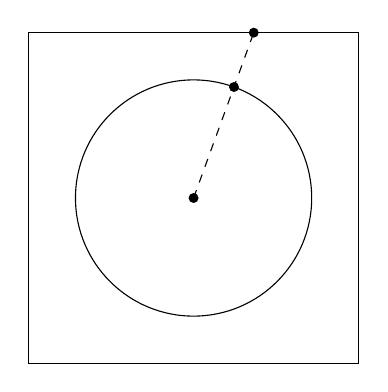
\begin{tikzpicture}[scale=1.5,>=latex]
  % Unit circle.
  \draw (0,0) circle (1);
  % Square circumscribing the circle (corners at (±1.4, ±1.4)).
  \draw (1.4,1.4) -- (-1.4,1.4) -- (-1.4,-1.4) -- (1.4,-1.4) -- cycle;
  % Origin.
  \fill (0,0) circle (1.2pt);
  % A sample point P on the circle (at angle 70°).
  \pgfmathsetmacro{\theta}{70}
  \pgfmathsetmacro{\px}{cos(\theta)}
  \pgfmathsetmacro{\py}{sin(\theta)}
  % Point Q on the square — radial projection of P.
  % For the upper edge y = 1.4, the ray from origin at angle θ hits
  % at x = 1.4 * cos(θ)/sin(θ) (assuming sin(θ) > 0 and within [-1.4, 1.4]).
  \pgfmathsetmacro{\qx}{1.4*cos(\theta)/sin(\theta)}
  \pgfmathsetmacro{\qy}{1.4}
  % Dashed ray from origin to Q (passing through P).
  \draw[dashed] (0,0) -- (\qx,\qy);
  % Mark P and Q.
  \fill (\px,\py) circle (1.2pt);
  \fill (\qx,\qy) circle (1.2pt);
\end{tikzpicture}
\end{document}
